\chapter{Evaluation}

As mentioned in Chapter 4 there is no reliable baseline and one needs to be established first with some basic CNN architectures. Then different architectures will be compared against each other with and without pre-training in order to find out if transfer learning is a valid option for this problem task. Data augmentation should add regularization and lead to a model that is better generalizable to the test set. New architectures will then be created to fit better the problem at hand. \\

The learning rate decay is defined as reducing the learning rate by a factor of 10 every N epochs, and holds true for all the experiments: \\

\[ lr = lr * (0.1^{\frac{epoch}{decay}}) \] \\

For the baseline I used a grid search approach in optimizing the learning rate and the learning rate decay. For all later architectures I used Sigopt which utilizes baysian optimization. With SIgopt I followed the official guideline to run the model for 10 times for every hyper parameter which needs to be optimized. For Alexnet and all state-of-the-art architectures I optimize the following three hyper parameters: learning rate [0.0001 - 0.1]; momentum [0 - 1]; weight\_decay [0.00001 - 0.01]. \\

Preliminary runs have shown that 50 epochs are long enough to converge as will be shown for every architecture seperately. \\

The remaining of this chapter is in the following format. I introduce the optimized hyper parameters for each architecture and show the achieved accuracies. I compare the results with transfer learning and disucuss the graphs and confusion matrices. For transfer learning a separate optimization with Sigopt is performed, since the hyper parameters need to be different if the starting point of the model is not randomly defined. Then I will will attempt to shed some light into what exactly was learned by showing some of the visualizations.

\section{CNN\_Basic - Baseline}

For the baseline a simple 3-layered CNN was chosen with three convolutions and no maxpooling. For the activation function a leaky ReLU is applied after each convolution. A simple grid search is applied on the model as seen in table \ref{tbl:cnn-basic-baseline}. The best result is achieved with a rather small learning rate of 0.0005 and a lr-decay of 20.

\begin{table*}[h]
	\ra{1.3}
    \caption{Accuracy (\%) for several learning rates and lr-decays for CNN\_Basic as a baseline.}
    \centering
    \begin{small}
	\textsc{
      \resizebox{0.99\textwidth}{!}{%
      \begin{tabular}{rcclcclcc}
      \toprule 
      & \multicolumn{2}{c}{Learning-Rate decay: 10} && %
        \multicolumn{2}{c}{Learning-Rate decay: 15} && %
        \multicolumn{2}{c}{Learning-Rate decay: 20} \\
      \cmidrule{2-3} \cmidrule{5-6}  \cmidrule{8-9}
      & learning rate & accuracy  && %
        learning rate & accuracy  && %
        learning rate & accuracy  \\ 
      \midrule
      CNN\_BASIC		& 0.1 & 69.10\%  &&  0.1 & 65.78\% &&  0.1 & 64.78\% \\
      CNN\_BASIC		& 0.05 & 63.46\%  &&  0.05 & 67.44\% && 0.05 & 65.78\% \\
      CNN\_BASIC		& 0.01 & 69.77\%  &&  0.01 & 70.10\% &&  0.01 & 69.77\% \\
      CNN\_BASIC		& 0.005 & 68.44\%  &&  0.005 & 71.43\% &&  0.005 & 72.09\% \\
      CNN\_BASIC		& 0.001 & 72.43\%  &&  0.001 & 70.10\% &&  0.001 & 74.42\% \\
      CNN\_BASIC		& 0.0005 & 73.75\%  &&  0.0005 & 73.42\% &&  \textbf{0.0005} & \textbf{76.74\%} \\
      CNN\_BASIC		& 0.0001 & 68.11\%  &&  0.0001 & 70.76\% &&  0.0001 & 70.43\% \\
    \bottomrule
    \end{tabular}}
	}
    \end{small}
    %\end{center}
    \vspace{-3.9mm}
    \label{tbl:cnn-basic-baseline}
\end{table*}

Although the accuracies look already very promising, it is not clear what the network learned. It could be some lightening that occur with asbestos samples or simply some other characteristics that have nothing to do with the asbestos itself. To be more aware of these issues several other outputs need to be included like a confusion matrix that shows how many true positives and false negatives are found.

\subsection{AlexNet}

AlexNet was optimized with grid search and additionally with sigopt. With the grid search the best accuracy is 81.06\% as seen in table \ref{tbl:alexnet-baseline}. It was achieved with a learning rate of 0.0001 and a learning rate decay of 20. Interestingly the SigOpt also achieved the same accuracy with a learning rate of 0.038984, momentum of 0.073145 and a weight decay of 0.004074 as seen in table \ref{tbl:alexnet-baseline}.


\begin{table*}[h]
	\ra{1.3}
    \caption{Accuracy (\%) for several learning rates and lr-decays for AlexNet as a baseline.}
    \centering
    \begin{small}
	\textsc{
      \resizebox{0.99\textwidth}{!}{%
      \begin{tabular}{rcclcclcc}
      \toprule 
      & \multicolumn{2}{c}{Learning-Rate decay: 10} && %
        \multicolumn{2}{c}{Learning-Rate decay: 15} && %
        \multicolumn{2}{c}{Learning-Rate decay: 20} \\
      \cmidrule{2-3} \cmidrule{5-6}  \cmidrule{8-9}
      & learning rate & accuracy  && %
        learning rate & accuracy  && %
        learning rate & accuracy  \\ 
      \midrule
      AlexNet		& 0.1 & 59.80\%  &&  0.1 & 59.80\% &&  0.1 & 60.47\% \\
      AlexNet		& 0.05 & 59.80\%  &&  0.05 & 59.80\% && 0.05 & 59.80\% \\
      AlexNet		& 0.01 & 59.80\%  &&  0.01 & 59.80\% &&  0.01 & 59.80\% \\
      AlexNet		& 0.005 & 59.80\%  &&  0.005 & 59.80\% &&  0.005 & 59.80\% \\
      AlexNet		& 0.001 & 74.75\%  &&  0.001 & 77.74\% &&  0.001 & 78.74\% \\
      AlexNet		& 0.0005 & 78.74\%  &&  0.0005 & 80.40\% &&  0.0005 & 76.74\% \\
      AlexNet		& 0.0001 & 74.75\%  &&  0.0001 & 80.07\% &&  \textbf{0.0001} & \textbf{81.06\%} \\
    \bottomrule
    \end{tabular}}
	}
    \end{small}
    %\end{center}
    \vspace{-3.9mm}
    \label{tbl:alexnet-baseline}
\end{table*}

\subsection{Transfer learning on AlexNet}

When using weights from pre-training on ImageNet, the overall accuracy does get slightly better, although the increase of 0.6645\% could be due to chance. In order to show if pre-training really helps with alexnet, each model has been run 5 times and the results are averaged. A t-test has been run to show it's significance [NEEDS TO BE DONE]

\begin{table}[h] \centering
\ra{1.3}
\caption{Hyper parameters for Alexnet optimized with SigOpt and without pre-training}
\resizebox{0.99\textwidth}{!}{%
\begin{tabular}{@{}rrrrrrr@{}}
\toprule & learning rate & momentum & weight\_decay & lr-decay & accuracy & $\Delta$ \\
\midrule
AlexNet	 from scratch	& 0.038498 & 0.073146 &  0.004074 & xxx & 81.0631\%  &		 \\
AlexNet	 pre-trained	& 0.034288 & 0.409378 &  0.005959 & xxx & 81.7276\%  & + 0.6645\\
\bottomrule
\end{tabular}}
\label{tbl:AlexNetBaseline}
\end{table}

In Figure \ref{fig:alexnet-graph} we see the training and validations accuries plotted over epochs. It can be observed that convergence is not faster with pre-training than without pre-training. Both final accuracies are almost identical. The gray vertical lines seperate the graph into segments with different learning rates. So the learning rate decay happens a first time at epoch 20 and a second time at epoch 40. Convergence can be easily obvserved when the validation accuracy does not change anymore. Another important thing to notice is that validation and training accuracies are quite near to each other. That simply means that during training no severe overfitting occured and that the validation set and train set are indeed very similar to each other. Since the final accuracy is also very near to these values it is save to say that validation and test sets are good representations of the test set and that generalizability has low variance [IF GENERALIZABILITY CAN HAVE A VARIANCE AT ALL... TODO: READ IT UP].

\begin{figure}[h]
\centering
\subfigure[Example with an asbestos fiber spanning from top to down]{
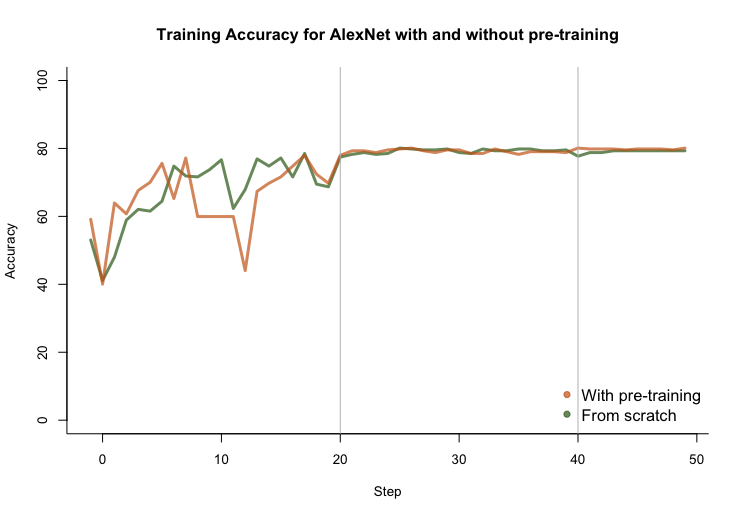
\includegraphics[width=.46\textwidth]{images/chapter5/TL/AlexNet/TA-AlexNet.png}
}
\subfigure[Example without any asbestos fibers]{
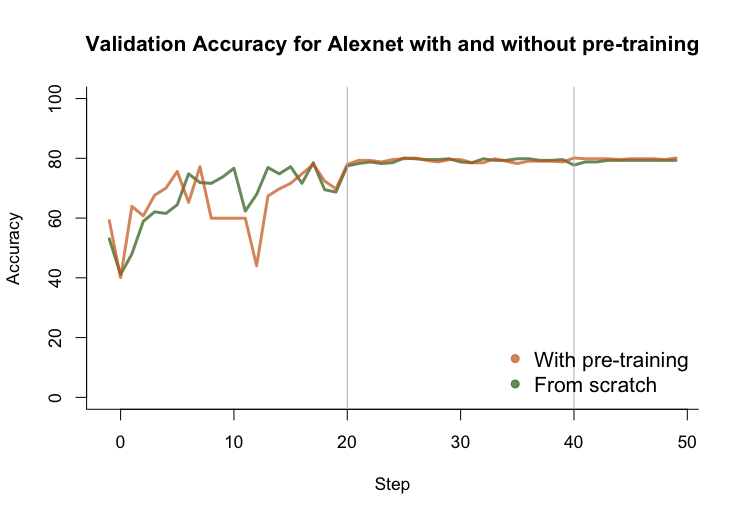
\includegraphics[width=.46\textwidth]{images/chapter5/TL/AlexNet/VA-AlexNet.png}
}
\caption{Some examples on how the microscopic images look like, and what kind of error in images occur.}
\label{fig:alexnet-graph}
\end{figure}

In Figure \ref{fig:alexnet-cm} the confusion matrix of the final test set is shown for both models (pre-trainend and non pre-trained). 

\begin{figure}[h]
\centering
\subfigure[Example with an asbestos fiber spanning from top to down]{
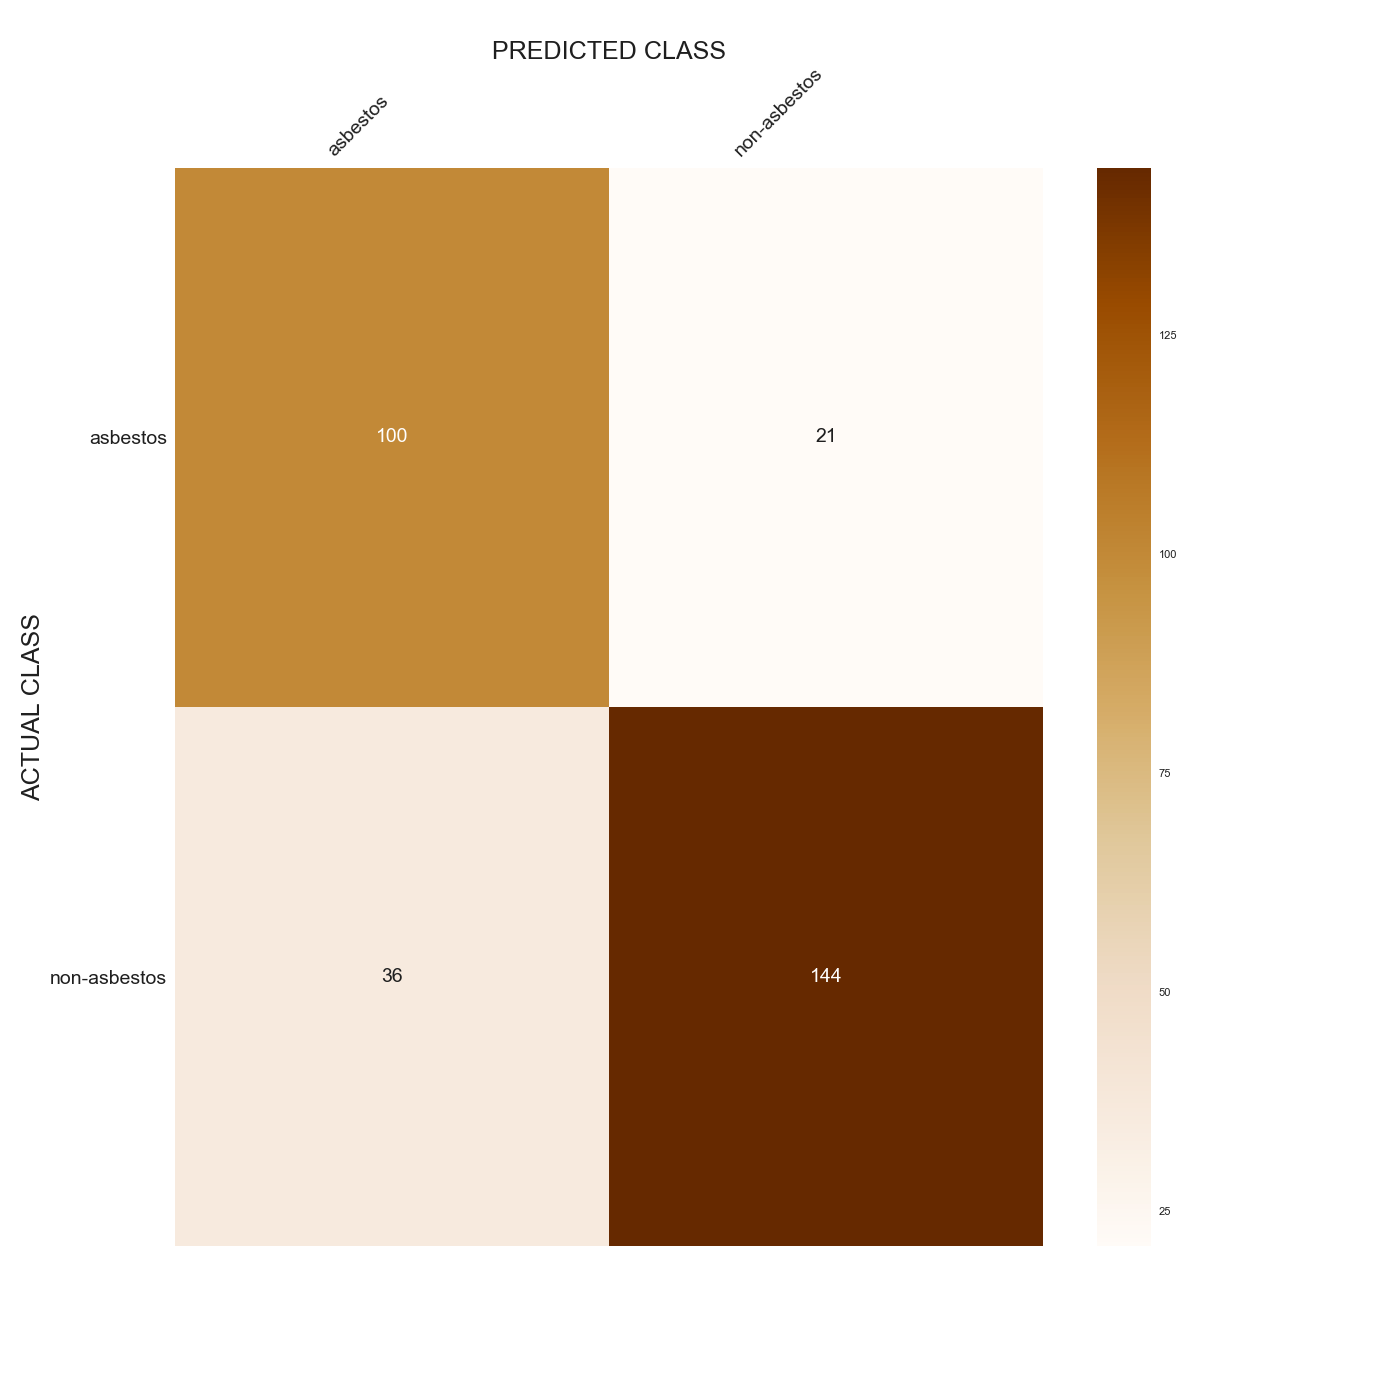
\includegraphics[width=.46\textwidth]{images/chapter5/TL/AlexNet/cm-alexnet.png}
}
\subfigure[Example without any asbestos fibers]{
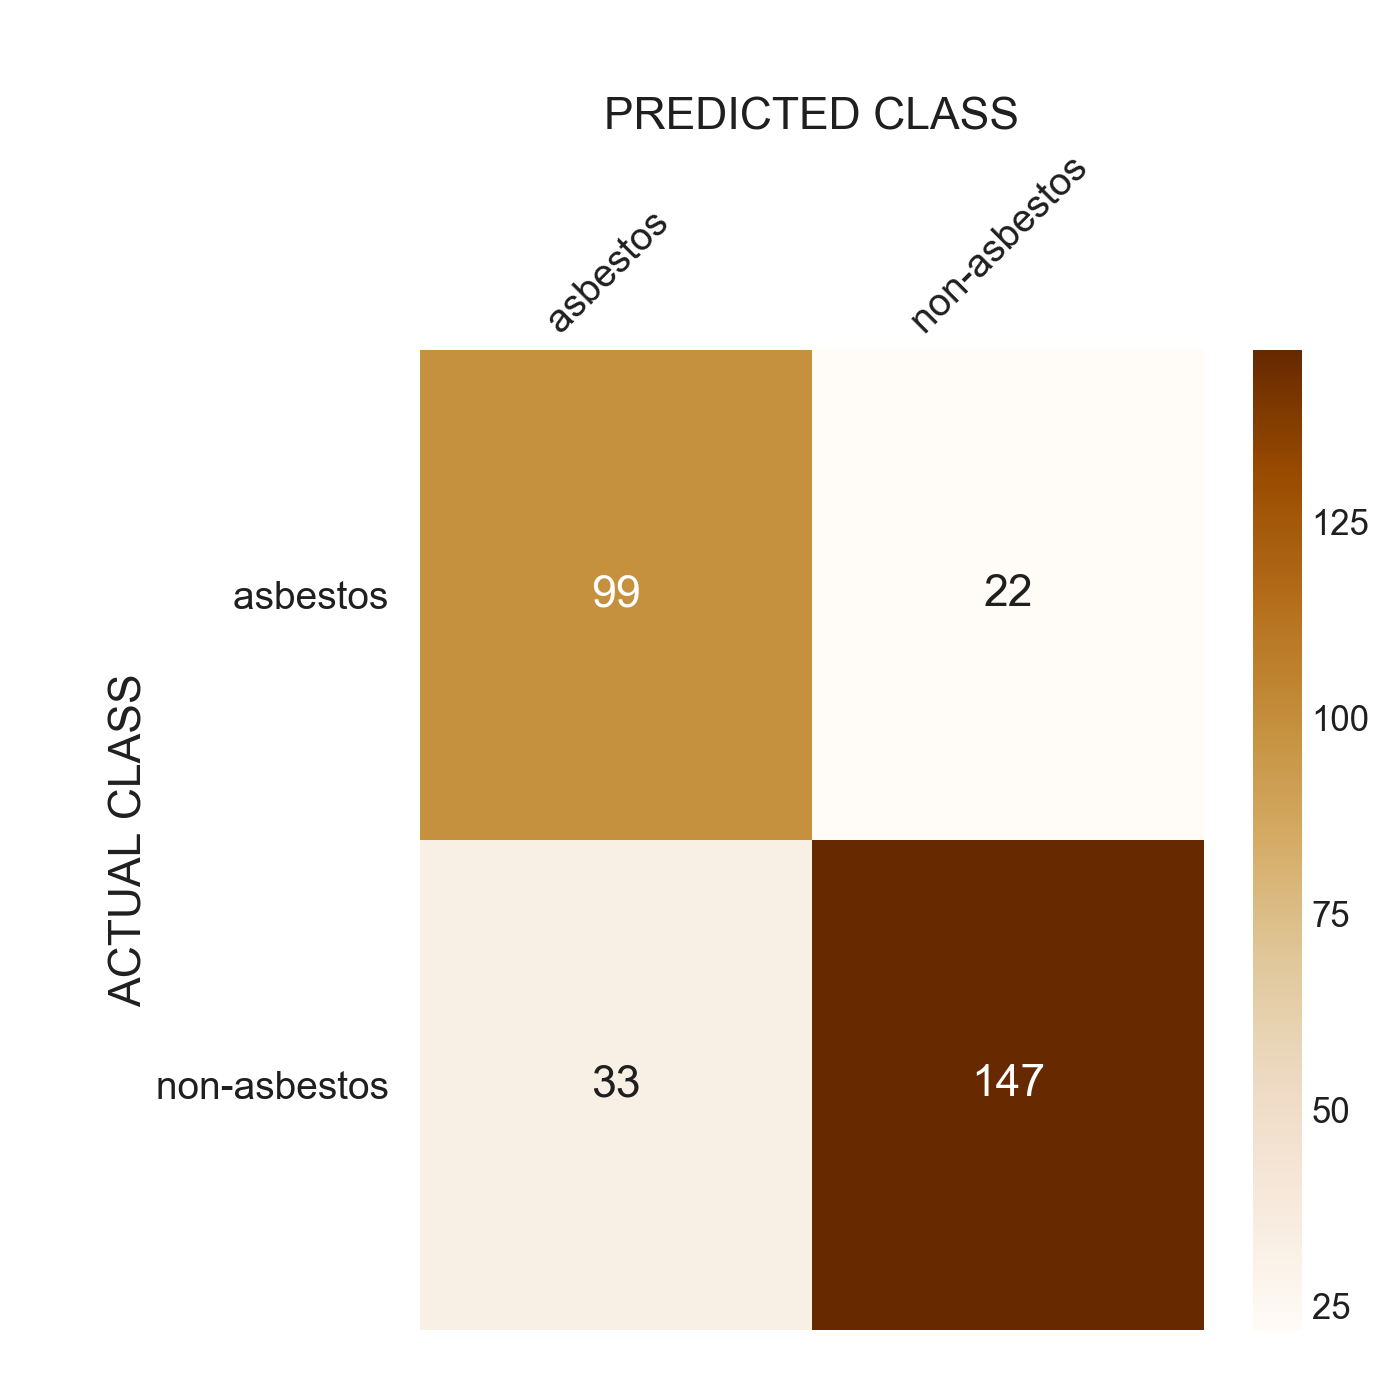
\includegraphics[width=.46\textwidth]{images/chapter5/TL/AlexNet/cm-alexnet-pre.png}
}
\caption{Some examples on how the microscopic images look like, and what kind of error in images occur.}
\label{fig:alexnet-cm}
\end{figure}


\section{ResNet18}

\section{Densenet}

\section{Inception}


